\setcounter{page}{1}
\renewcommand{\thepage}{\arabic{page}}

\subsection*{付録 A: \eqref{eq:ptemp_entropy_relation_ingeneral} の導出に関する補足}
\begin{wrapfigure}{l}{0.45\linewidth}
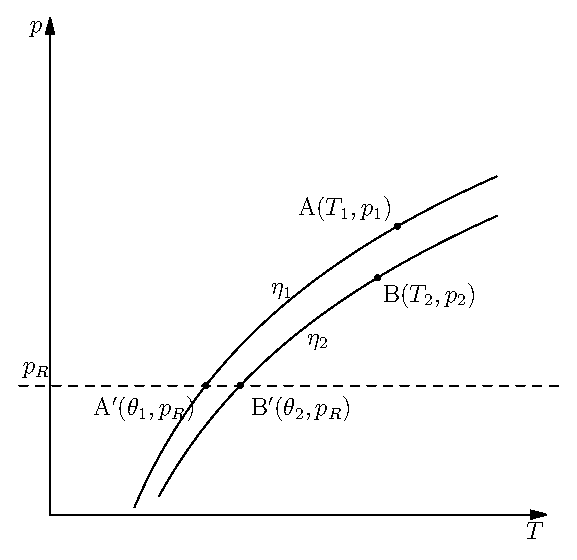
\includegraphics[width=\linewidth]{./appendix_Fig1}
\caption{\footnotesize 状態 A から状態 B に変化したときのエントロピーの微小変化$d\eta (= \eta_2-\eta_1)$を考える.}
\label{fig:appendix_Fig1}
\end{wrapfigure}
% % % % % % % % % % % % % % % % % % % % % % % % % %
エントロピーの変化と\eqref{eq:PTemp_generalDef}で定義される温位の変化の関係式の導くために, 
任意の状態$(T_1,p_1)$から任意の状態$(T_2,p_2)$に変化したときのエントロピーの微小変化$d\eta$を考えよう.
それぞれの状態は, 図\ref{fig:appendix_Fig1}において点 A, B に対応している. 

エントロピーを温度と圧力の関数とするとき, その微小変化は, 
\begin{equation*}
 (d\eta)_{{\rm A}\to{\rm B}} = \DP[][T]{\eta}{p} (dp)_{{\rm A}\to{\rm B}} + \DP[][p]{\eta}{T} (dT)_{{\rm A}\to{\rm B}}
\tag{A.1}
\end{equation*}
と書ける. 
添字${\rm A}\to{\rm B}$は, 状態 A から状態 B へ変化したときの微小変化であることを示している. 
エントロピーと温位の微小変化の関係式を導くには, (A.1) の右辺の
$(dp)_{\rm A \to B}, (dT)_{\rm A \to B}$を, \eqref{eq:PTemp_generalDef}の定義を使って$(d\theta)_{\rm A \to B}$に
書き換えなければならない.  
もし, 実直に\eqref{eq:PTemp_generalDef}の両辺の変分をとることにより 
\eqref{eq:ptemp_entropy_relation_ingeneral}を導くならば, やや複雑な計算が必要である%
\footnote{
\eqref{eq:PTemp_generalDef}の両辺の変分をとることにより 
\eqref{eq:ptemp_entropy_relation_ingeneral}を導く場合を考えよう. 

$T,p$を独立変数として\eqref{eq:PTemp_generalDef}の両辺の変分を取り, 変形すれば, 
\begin{align*}
 dT = \left[ d\theta + \DP[][\eta]{T}{p} dp \right] \left[ 1 + \int_{p}^{p_R}  \DP{}{T} \DP[][\eta]{T}{p^\prime} (T,p^\prime) dp^\prime \right]^{-1} 
\end{align*}
を得る. 
積分を含む因子を$I(p,T,p_R)$で表して, (A.1) の右辺に代入し整理すれば, 
\begin{align*}
 d\eta &= I\DP[][p]{\eta}{T} \; d\theta 
        + \left[ \DP[][T]{\eta}{p} + I \DP[][p]{\eta}{T} \DP[][\eta]{T}{p}  \right] dp  \\
       &= I \DP[][p]{\eta}{T} \; d\theta 
        + \left[ \left( 1-I \right)\DP[][T]{\eta}{p} \right] dp. 
\end{align*}
後は本文と同様の議論をすれば良い. 
なお, $p=p_R$の圧力一定の過程では$I=1$となることに注意されたい. 
}. 
代わりに, 次のように考えるとエントロピーと温位の微小変化の関係式を簡単に導ける. 

点 A, B 間のエントロピーの変化を,
代わりに$p=p_R$上の点 A$^\prime$, B$^\prime$間で考えることにしよう. 
点 A$^\prime$, B$^\prime$間で圧力一定の過程を考えるとき, 
その過程における温度は定義により温位である. 
したがって, 
点 A$^\prime$, B$^\prime$間のエントロピーの微小変化は, 
\begin{equation*}
 (d\eta)_{{\rm A^\prime}\to{\rm B^\prime}} = \dfrac{c_p(p_R,\theta)}{\theta} (d\theta)_{{\rm A^\prime}\to{\rm B^\prime}}
\tag{A.2}
\end{equation*}
と書ける. 
ただし, 定圧比熱の定義を用いた. 
また, 点 A$^\prime$, B$^\prime$はそれぞれ, 点 A, Bと同じ等エントロピー線$\eta_1, \eta_2$上にあるので, 
$(d\eta)_{\rm A \to B} = (d\eta)_{\rm A^\prime \to B^\prime}, \;
(d\theta)_{\rm A \to B} = (d\theta)_{\rm A^\prime \to B^\prime}$
が成り立つ. 
したがって,  
\begin{equation*}
 (d\eta)_{\rm A\to B} = \dfrac{c_p(p_R,\theta)}{\theta} (d\theta)_{\rm A \to B}
\tag{A.3}
\end{equation*}
を得る. 


